\documentclass{article}
\usepackage[utf8]{inputenc}
\title{Lecture 10 low rank models}
\author{wbg231 }
\date{December 2022}
\newcommand{\R}{$\mathbb{R}$}
\newcommand{\B}{$\beta$}
\newcommand{\A}{$\alpha$}
\newcommand{\D}{\Delta}

\newcommand{\avector}[2]{(#1_2,\ldots,#1_{#2})}
\newcommand{\makedef}[2]{$\textbf{#1}$:#2 }
\usepackage{tikz,graphicx,hyperref,amsmath,amsfonts,amscd,amssymb,bm,cite,epsfig,epsf,url}

\begin{document}

\maketitle

\section*{introduction}
\begin{itemize}
\item the prof stopped making videos so form now on these are going to be text book notes 
\item \href{https://brightspace.nyu.edu/content/enforced/249915-794-1234_SP23DS-GAMATH-GA28403001005/notes/pca.pdf}{link}
\item up to now we have seen datasets where each data point is associated with a single entity 
\item now we are going to talk about cases where the data set are associated with two different entities
\item we represent such data as entries in a matrix $D$ for each enters $D[i,j]$ column i row j indicate the entries associated to each data point 
\item for example in recommender systems $D[i,j]$ would correspond to the rating user i gave to product j. 
\item for example in genomics $D[i,j]$ would correspond to the expression of gene i in cell j 
\item also i may use $D[i,j]$ and $D_{i.j}$ interchangeably 
\item in order to analyze such data it is often useful to represent each data point in terms of a small number of factors. 
\item this can be done by fitting the data using a low rank approximation 
\subsection*{movie example}
\item consider a matrix of movie rating $D\in \mathbb{R}^{n_1\times n_2}$ where $D_{i,j}$ is the rating user i gave to movie j 
\item to model $D$ we approximate $D_{i,j}$ as a sum of r components where $r\leq min{n_1,n_2}$ (recall that the max number of 
eigenvalues the matrix $A\in \mathbb{R}^{n\times d}$ is min(n,d) that is the number of linearly independent rows and columns so if we use more than that number of components it is not a low rank model )
\item let the lth component be the produce of a coefficient $a_{l}[i]$ associated to movie i and a coefficient $b_{l}[j]$ associated to user j thus we have 
approximation of the matrix given by $$L[i,j]=\Sigma_{l=1}^{r}a_{l}[i]b_{l}[j], \quad \forall i\in [1,n_1], j\in [1,n_2]$$
\item so keep in mind that what we have effectively is $$L\in \mathbb{R}^{n_1\times n_2}=
\begin{pmatrix}
a_1 & a_2 & \cdots & a_r    
\end{pmatrix}\begin{pmatrix}
    b_1 \\ b_2  \\ \cdots \\ a_r    
    \end{pmatrix}=AB\approx D\in \mathbb{R}^{n_1\times n_2}: \forall a_i\in A a_i\in \mathbb{R}^{n_1},b_i\in B b_i\in \mathbb{R}^{n_2}$$
\item think of $a_{l}[i]$ as indicating wether the association of user i to factor l is positive negative or negligible. 
\item the model is bilinear because the approximation is a bilinear function of teh coefficients. if we fix either the user or movie coefficients the model is linear 
\item the rank of matrix $L$ is equal to r. this can be seen as $rank(AB)=min(rank(A), (rank(b)))=min(min(n_1,r), min(min(r,n_2))\leq r$ so if we select our component vectors to be linearly independent this will holds
\item given that r is much smaller than the rank of D this is known as a low rank model. 
\item these models are fit using SVD which decomposes any matrix into rank 1 components
\subsection*{low rank models and PCA}
\item in a low rank model each column of $L[i]=A_{i}^{T}B_{i}$ that is a linear combination of basis vectors
\item think of  $D\in \mathbb{R}^{n_1\times n_2}=\{D_{1},\cdots D_{n_2}\}$ that is a set of $n_1$ dimensional data points 
\item from here we can reduce there dimensionality to r by using pca
\begin{enumerate}
    \item we can write each of the $n_2$ columns of $D$ as $D[:,j]\in \mathbb{R}^{n_1}$
    \item first we can find the covariance matrix of columns of D as  $$\Sigma_{cols}=\frac{1}{n_2}\Sigma_{j=1}^{n_2}D[:,j]D[:,j]^t=\frac{1}{n_2}DD^{T}$$
    \item take the eigenvectors associated with the top $r$ largest eigenvalues tp obtain our principle directions
    \item project the matrix onto the those r principle directions to get r principle components $$w_{l}(j)=u_{l}^{t}D[:,j] \quad \forall j\in [1,n_2] $$ where $u_i$ is the ith principle direction of $\Sigma_{col}$ and 
    \item thus the set $\{w_{1}\cdots w_{r} \}$ representing $D\in \mathbb{R}^{r\times n_2}$
    \item and finally we can project back to our original space to get the low rank model $L_{pca-cols}[i,j]:=\Sigma_{l=1}^{r}u_{l}[i]w_{l}[j] \forall i\in [1,n_1], j\in [1,n_2]$
\end{enumerate}
\item this model is optimal from the point of preserving mean squared $\ell_{2}$ norm of the columns of D
\item alternatively we could conduct the same operation on the rows of $D$ in order to obtain the low rank model $L_{pca-rows}$
\item we will now show that these approaches are equivalent 
\subsection*{the singular value decomposition }
\item the SVD is a fundamental tool in linear algebra which decomposes a matrix into the product of a matrix with orthonormal columns
a diagonal matrix and a matrix with orthonormal rows. 
\item \textbf{SVD} allows us to decomposes any matrix $A\in \mathbb{R}^{n_1\times n_2}$ such that $n_1\leq n_2$ (if not we can 
take the transpose and this will hold) with rank t to its singular value from as \\
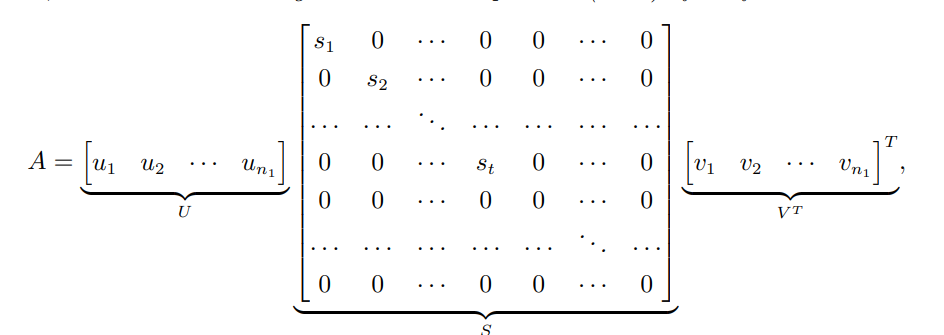
\includegraphics[width=10cm]{/home/buzgalbraith/work/school/spring_2023/probaility-theroy-2-2023/notes/week_10/video_!/images/v10_1.png}
\\ where  the singular values $s_1\geq s_2 \geq \cdots \geq s_t$ are positive real numbers, the left singular vectors
$u_1,u_2\cdots u_r\in \mathbb{R}^{n_1}$ are orthonormal and the right singular vectors $v_1,v_2\cdots v_r\in \mathbb{R}^{n_2}$

\item proof
\begin{enumerate}
    \item first it is clear that for an arbitrary matrix $A\in \mathbb{R}^{n_1\times n_2}$ we can write a symmetric matrix as $M:=AA^{T}\in \mathbb{R}^{n_1\times n_1}$
    \item and further by the spectral theorem we know that any symmetric matrix can be eiegen decomposed and thus has $n_1$ orthonormal vectors $u_1,\cdots , u_{n_1}$
    \item further note that the corresponding eigenvalues $\lambda_{n_1}$ are non-negative since $0> ||A^{t}u_{j}||_{2}^{2}=u_{j}^{t}AA^{t}u_{j}=u_{j}^{t}Mu_{j}=\lambda_{j}u_{j}^{t}u_{j}=\lambda_{j}$ that is positive definite
    \item and further the number of non-zero eigenvalues is equal to teh rank of A, and further because A and $AA^{T}$ have he same rank  
    \item the  number of non-zero eigen values of $m$ is equal to the rank of a, and since A and $A^{t}$ have the same number of eigenvalues call if $t$ we have $s_{t}:=\sqrt{\lambda_{t}}$ and $$v_{t}:=\frac{1}{s_{t}}A^tu_{1}$$
    \item further these vectors have unit norm $$||v||_{2}^{2}=\frac{1}{s_{1}^2}u_{1}^{t}AA^{T}u_{1}=\frac{\lambda _t}{\lambda_t}u_{1}^{T}u_{1}=1$$
    \item further all the singular vectors are orthogonal
    \item so we can define the fallowing matrices $$U:[u_1\cdots u_{n_1}]$$ $$V:[v_1\cdots v_{n_1}]$$ such that $$U^TA=SV^T$$
    notice here that U is orthogonal  matrix as it is square an has orthomonal columns thus $UU^{T}$ meaning that $$A=USV^T$$
\end{enumerate}
<<<<<<< HEAD
<<<<<<< HEAD
\item the rank of a matrix is equal to the number of non singular eigenvalues
\item we can write any matrix as a linear combination of rank 1 matrices as $$D=\Sigma_{l=1}^{n_1}S_{i}K_{l}=\Sigma_{l=1}^{n_1}s_{l}u_{l}v_{l}^{T}$$
\item the rank of matrix $K_{l}$ is one because it is the outter product of the left singular vector $u_{l}$ and the right singular vector $v_{l}$ so its ellements are scalled coppies of the two. 
\item the rank 1 matrices are orthogonal and have unit norm 
=======
>>>>>>> parent of 7708081 (Updates from Overleaf)
=======
>>>>>>> parent of 7708081 (Updates from Overleaf)
\item 
\end{itemize}
\end{document}
